\indent\indent When starting a new analysis, the software asks for an image to start with. Images from the same type present in the folder will be automatically selected and listed. Unselect images which shouldn't be part of the analysis, give your analysis a name and the grid creation tool will start.\\

\begin{figure}[!h]
   \centering
   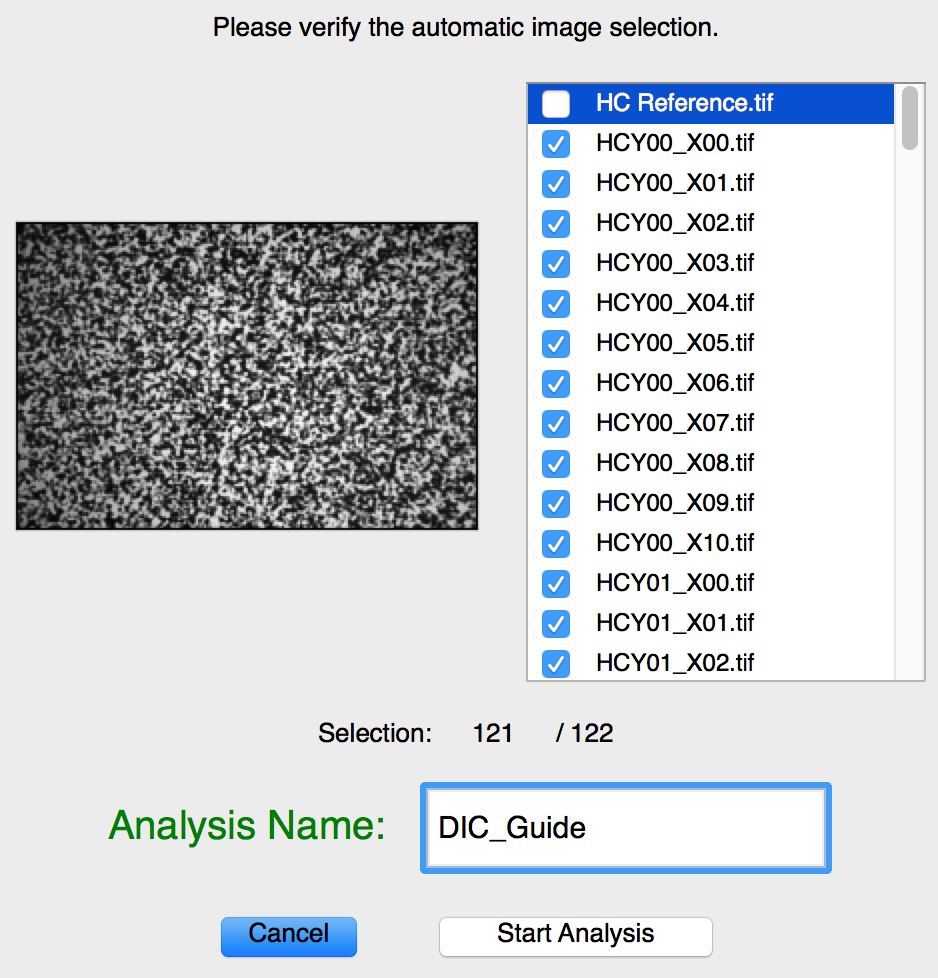
\includegraphics[scale=.4]{image_selection}
   \caption{New Analysis: Image Selection}
\end{figure}

\newline
\indent\indent The grid creation tool is divided into three main areas. The top part provides tools to build a grid necessary for the correlation process. Under this tools zone, the application is separated in two entities : the left side displays your images and the grid, the right side takes care of filters for your images.\\
\newpage
